  
\chapter{Results}
To test the software, the two stations were situated one outside the Electric and Electronic labs at Stellenbosch University and the other inside, with the UART giving the output as follows:
\definecolor{mygreen}{rgb}{0,0.6,0}
\definecolor{mygray}{rgb}{0.5,0.5,0.5}
\definecolor{mymauve}{rgb}{0.58,0,0.82}
\definecolor{terminalbgcolor}{HTML}{330033}
\definecolor{terminalrulecolor}{HTML}{000099}
\lstset{
	backgroundcolor=\color{terminalbgcolor},
	basicstyle=\color{white}\fontfamily{fvm}\footnotesize\selectfont,
	breakatwhitespace=false,  
	breaklines=true,
	captionpos=b,
	commentstyle=\color{mygreen},
	deletekeywords={...},
	escapeinside={\%*}{*)},
	extendedchars=true,
	frame=single,
	keepspaces=true,
	keywordstyle=\color{blue},
	%language=none,
	morekeywords={*,...},
	numbers=none,
	numbersep=5pt,
	framerule=2pt,
	numberstyle=\color{mygray}\tiny\selectfont,
	rulecolor=\color{terminalrulecolor},
	showspaces=false,
	showstringspaces=false,
	showtabs=false,
	stepnumber=2,
	stringstyle=\color{mymauve},
	tabsize=2
}
\begin{figure}[!htb]
\begin{lstlisting}
Bytes received: 80
SATELLITE time: 2023/5/16-21:55:57 Location: -33.9286628330, 18.8670256670 CO2:  +469.00,
MassConcentrationPm1p0:  +3.60,MassConcentrationPm2p5: 3.80,MassConcentrationPm4p0: 3.80,
MassConcentrationPm10p0: 3.80,AmbientHumidity: 86.72,AmbientTemperature: 10.62C,
VocIndex: 19.00,NoxIndex: 1.00
\end{lstlisting}
\end{figure}

\noindent
This shows the received contents from the satellite station, as well as the size of the bytes received. This confirms the transfer system working as expected. With this confirmed, the next test was to see if the WiFi download server was working on the base station and if the data had been written to the SD card.

\begin{figure}[!htb]
	\minipage{0.4\textwidth}%
	\includegraphics[width=\textwidth]{body/fig/ESPServer}
	\caption{Main page for website}
	\label{fig:espserver}
	\endminipage\hfill
	\minipage{0.4\textwidth}%
	\includegraphics[width=\textwidth]{body/fig/datacsvshow}
	\caption{data.csv file present on the SD card and accessible through the URL}
	\label{fig:datacsvshow}
	\endminipage\hfill
\end{figure}

\noindent
In order to access the data locally, if a database or API was not set up, the ESP32-S2 hosts a file server that grants access to all the files on the SD card. The HTML file for the server is also located on the SD card. When the user wishes to view the data for the various stations, they go to the base IP address as designated by the router attached, type forward slash $<$File Name$>$ -in the case of the base station and first satellite this would be data.csv and data1.csv. As seen in Figure~\ref{fig:datacsvshow} the data was accessible from the web portal when connected to the WiFi access point.

\begin{figure}[!htb]
	\centering
	\includegraphics[width=0.5\linewidth]{body/fig/speed}
	\caption{Speed of download is about 270kB/s }
	\label{fig:speed}
\end{figure}

\noindent
When measuring the speed of the download using the local network, the data was downloaded at about 270 kB/s, this would mean a day's data would take about four seconds to download. This means the system is capable of providing data to an outside entity at sufficient speeds should it need to, like a database.


%First say what you are looking at. Then say what yo get from figure
%now given this what does it tell you
%for each table and figure

%\end{figure}
\begin{figure}[!htb]
	\centering
	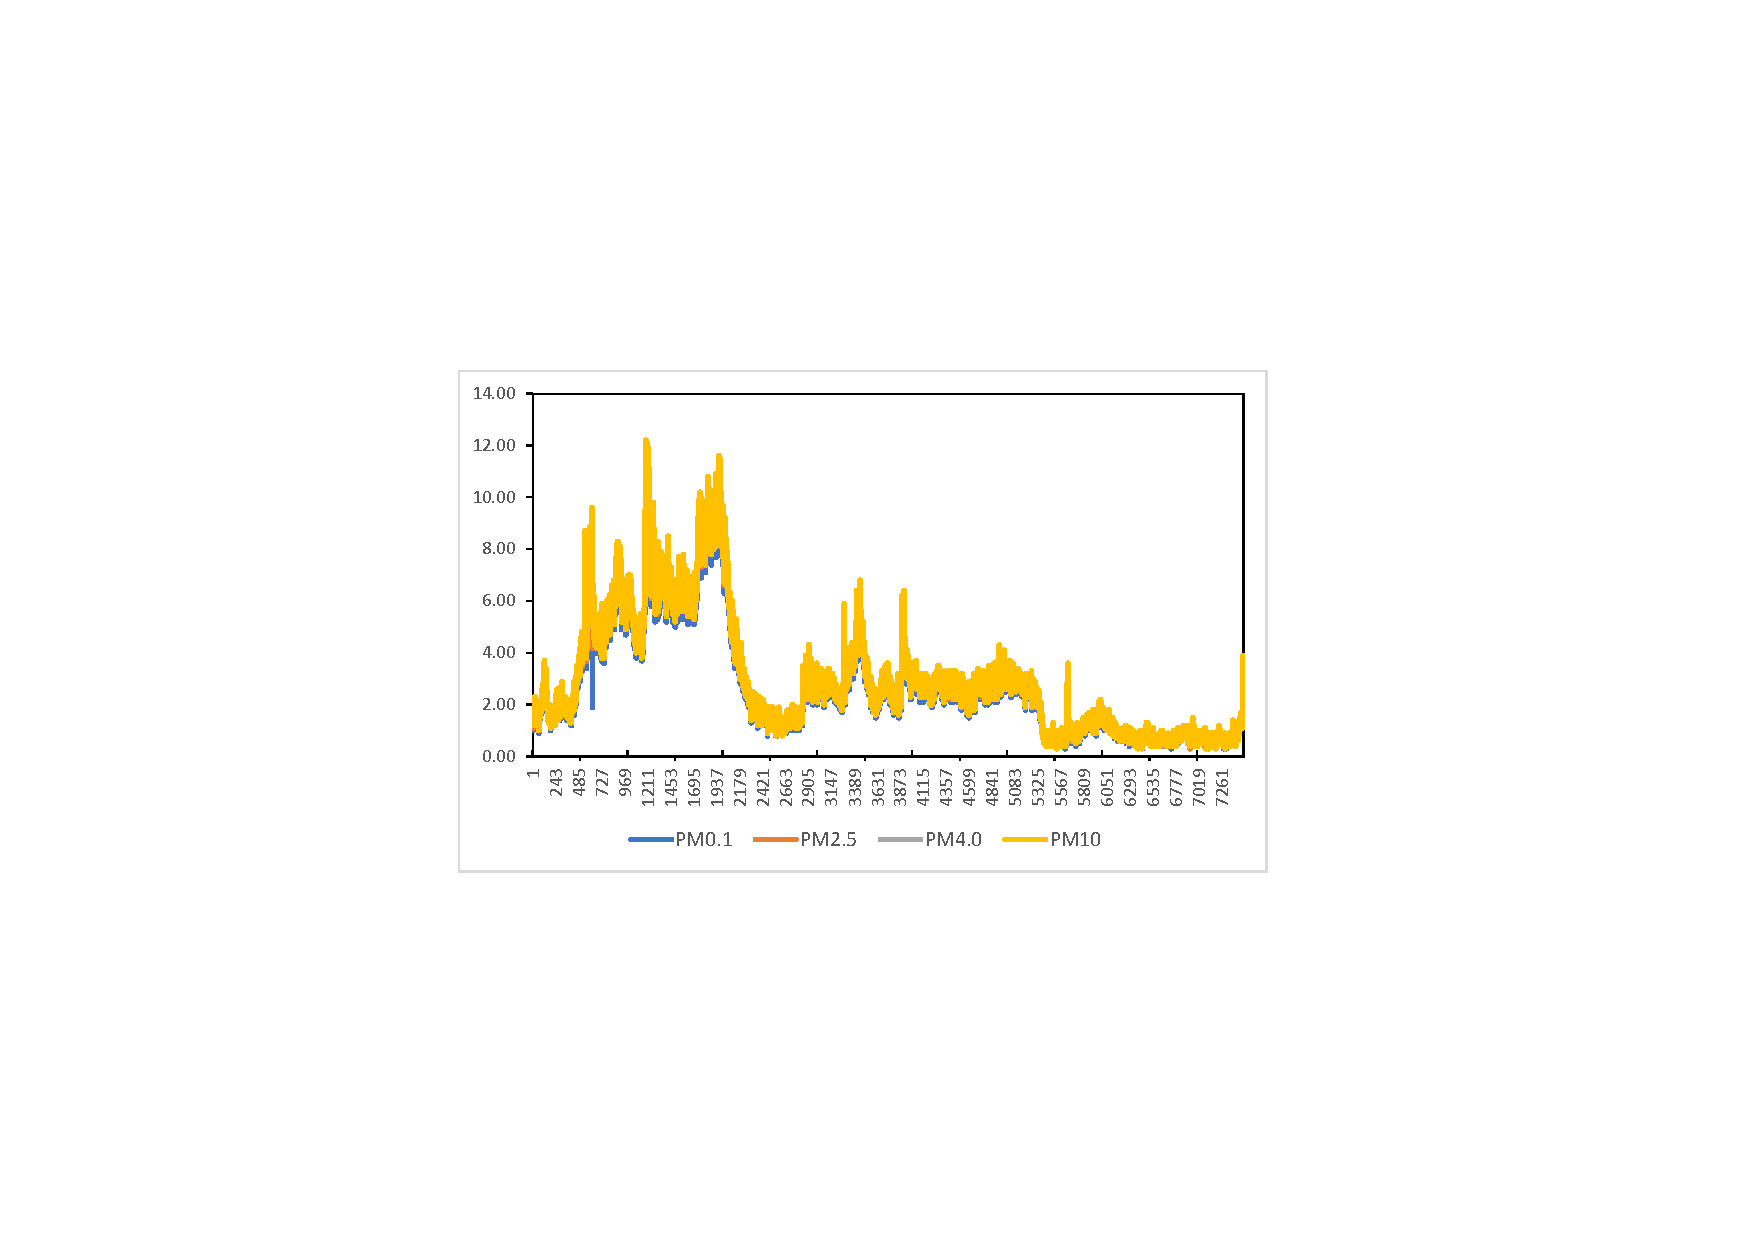
\includegraphics[width=0.9\linewidth]{body/fig/PMall2.0.pdf}
	\caption[Particulate Matter]{Particulate Matter graph of 7000 data points at all concentrations measured.}
	\label{fig:PMall}
\end{figure}

\noindent
In order to see if the data was reliable, the devices were set up in a stationary spot for nearly 24 hours. After the initial settling times for all the measurements, both stations showed nearly identical graphs, this marked the data as relatively reliable.
The correlation between all the different sizes of particulate matter concentrations was rather high, as can be seen from Figure~\ref{fig:PMall}, this means that conceivably only  the PM 2.5 reading could be used to indicate the quality as is the norm in the industry. The rough timing of the chart is late afternoon to the next day, with the elevated period in the middle representing the evening.
The peaks at the start are the testing of the sensor with various methods while it was on the testing desk.
In order to test the various sensors, pure CO2 from a small CO2 gas canister was used to test if the sensor was responding with relative accuracy and in a timely manner.


\begin{figure}[!htb]
	\centering
	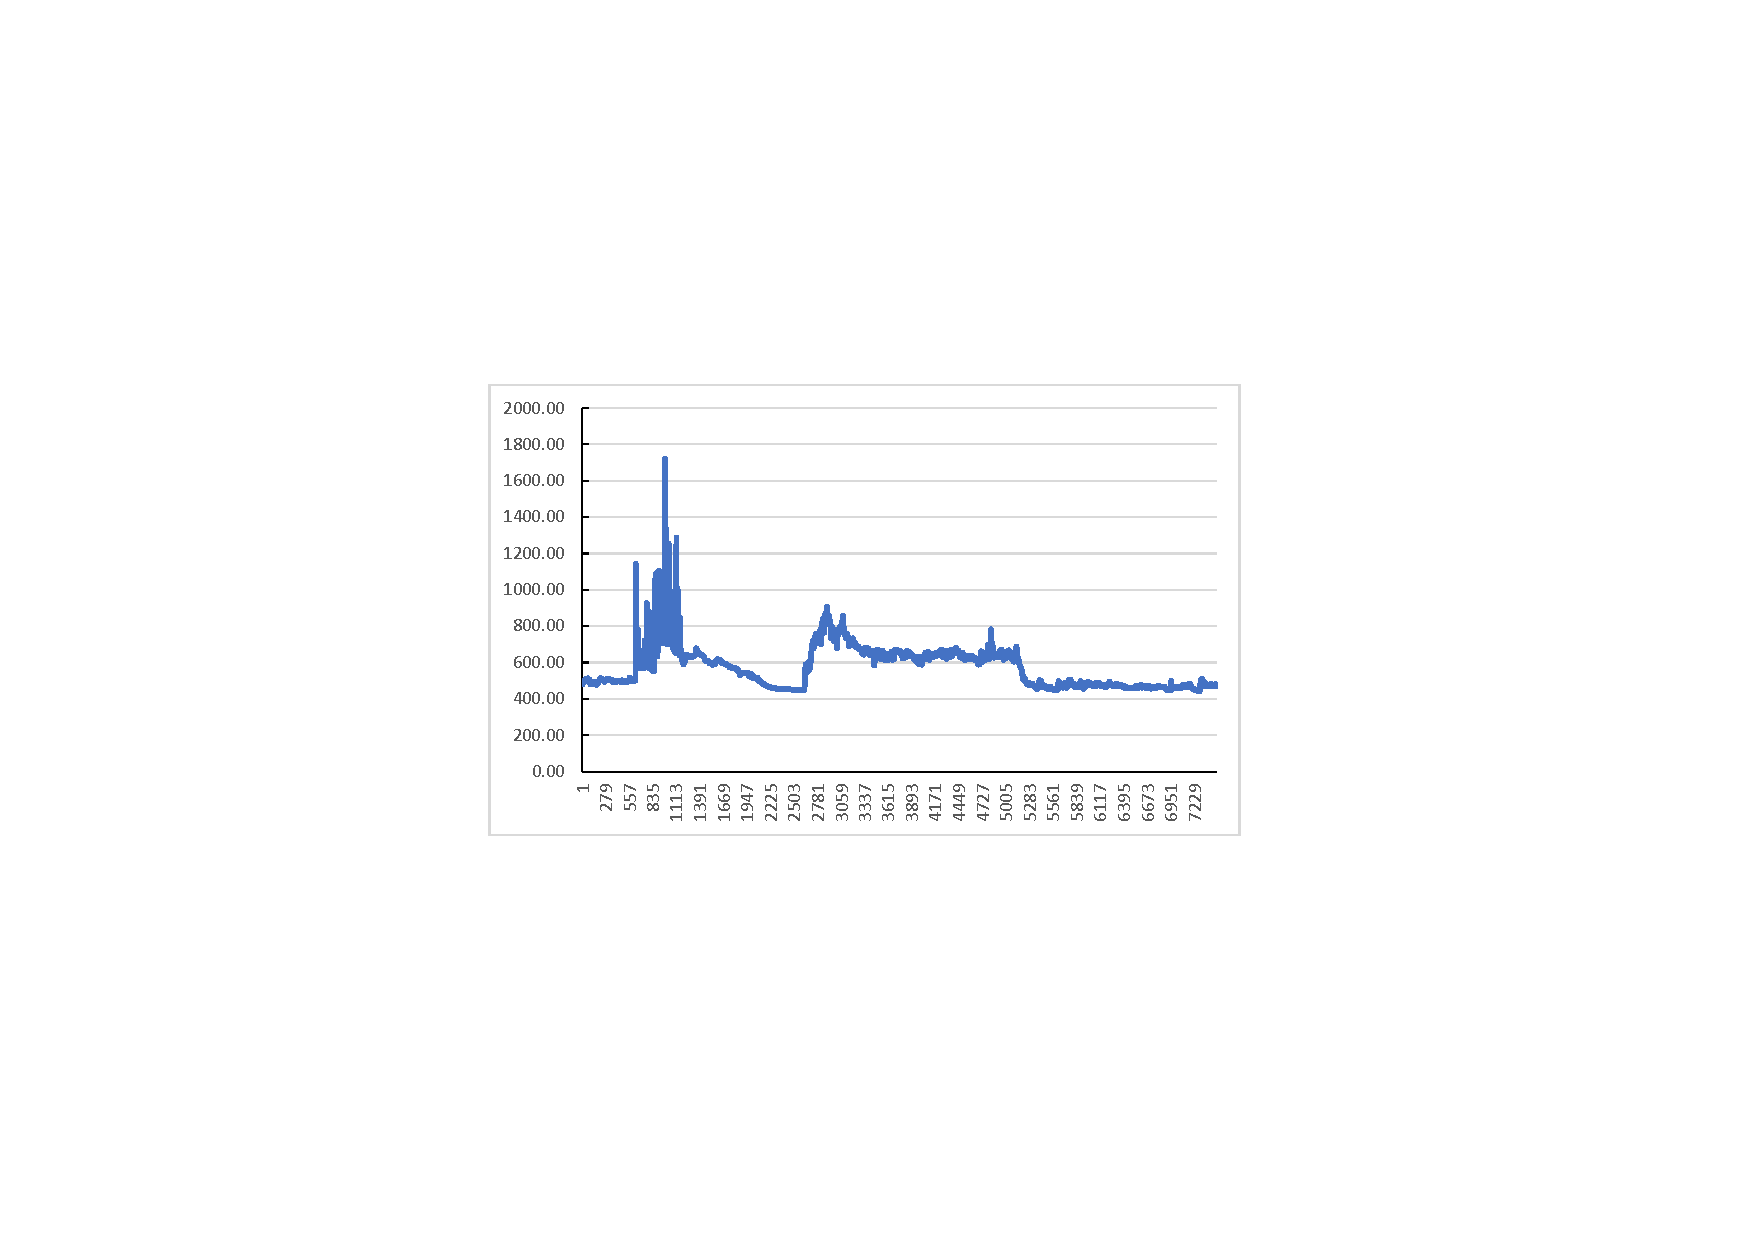
\includegraphics[width=0.7\linewidth]{body/fig/CO22.0.pdf}
	\caption{CO2 measurements}
	\label{fig:co2}
\end{figure}

\noindent
In Figure~\ref{fig:co2} the CO2 concentration is shown for the same period. The CO2 reading is much more consistent and is also much quicker to respond and settle, it has a near instant response to elevated levels and could be a good indicator of immediate air quality loss.%here the concentration is much more discernable, with the CO2 remaining consistent and lowering through the night as lighter breathing and less activity realises a slightly less steep than the initial start, the dips in-between are when there was no one inside the testing area.


\begin{figure}[!htb]
	\minipage{0.45\textwidth}%
	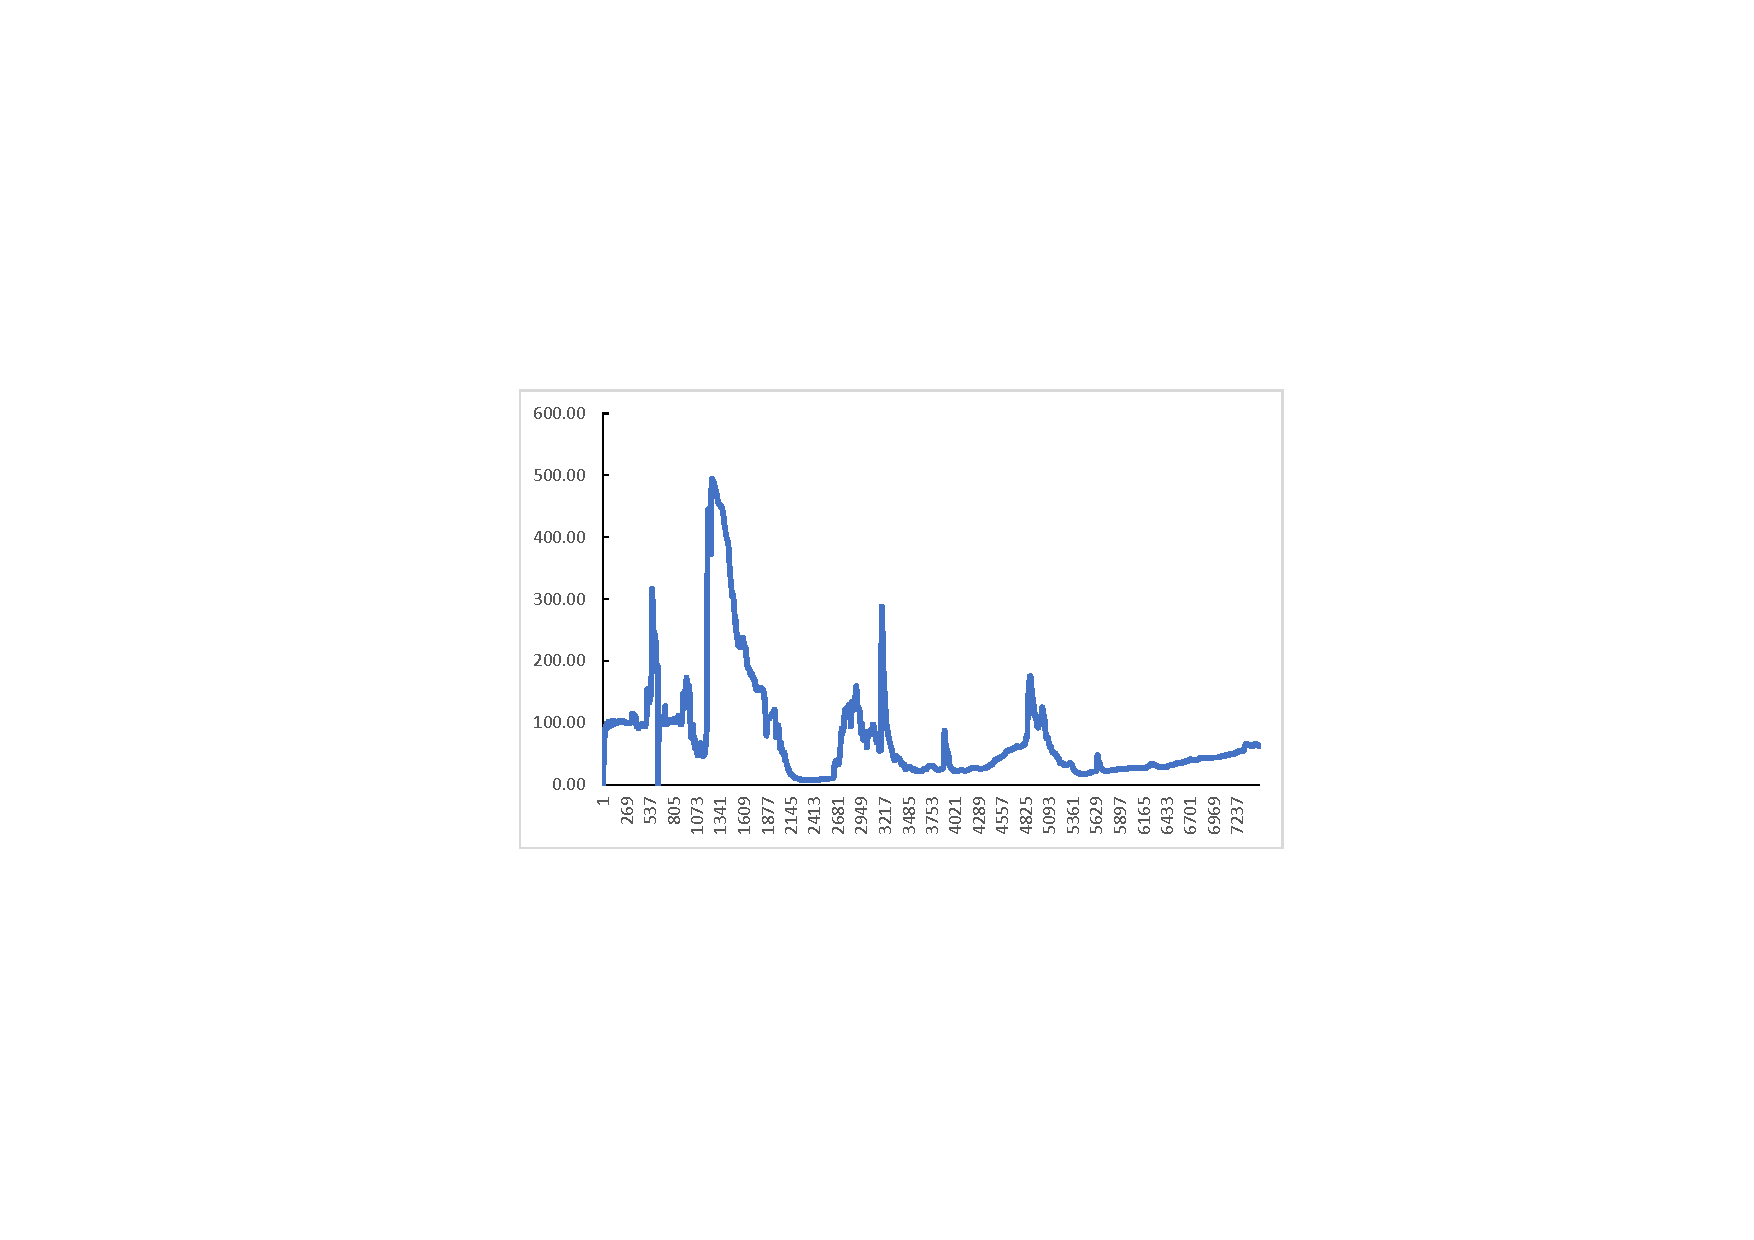
\includegraphics[width=\linewidth]{body/fig/VOC2.0.pdf}
	\caption{VOC}\label{fig:voc}
	\endminipage\hfill
	\minipage{0.45\textwidth}%
	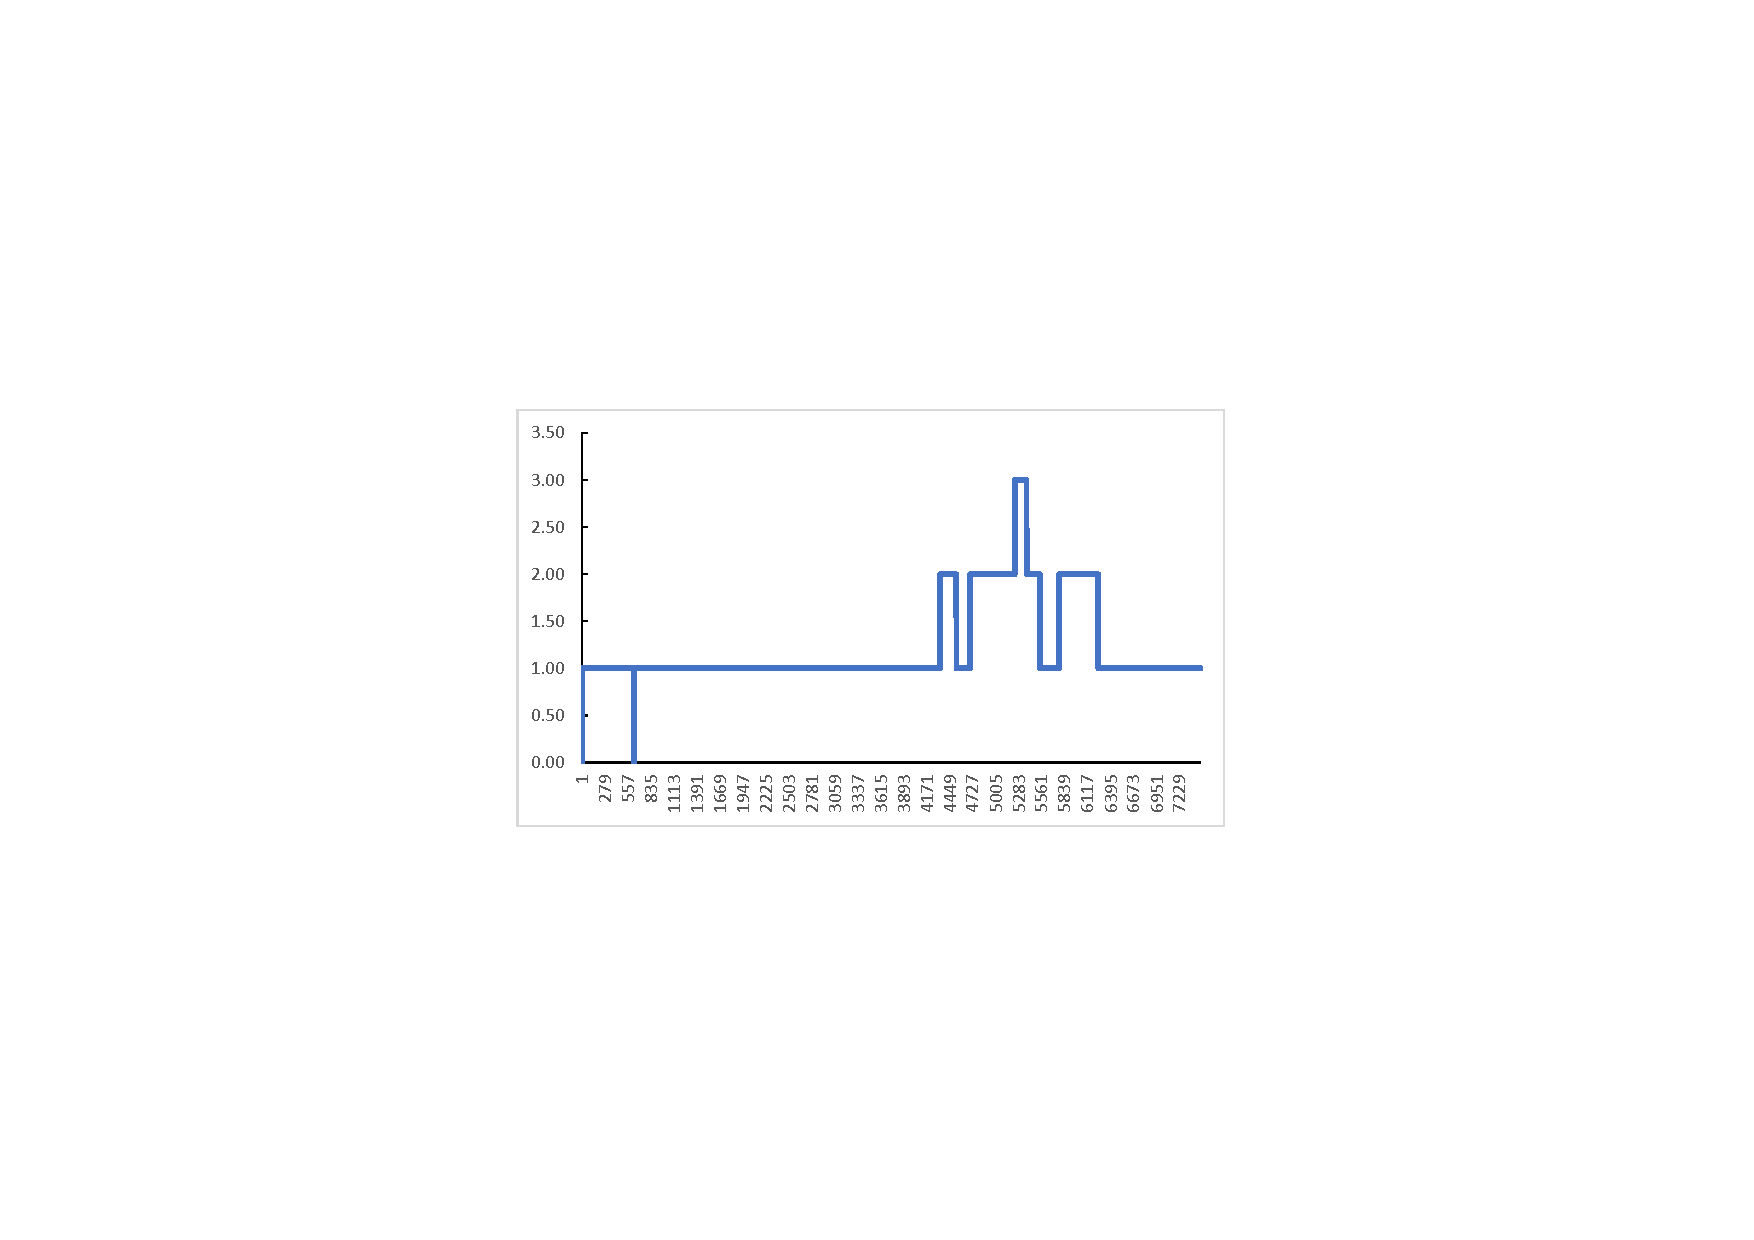
\includegraphics[width=\linewidth]{body/fig/NOX2.0.pdf}
	\caption{NOx}\label{fig:nox}
	\endminipage\hfill

\end{figure}

\noindent
VOC and NOx readings spiked along with the other test samples and as mentioned in the section, the NOx readings only become viable after a few hours, with it also moving up a few index points, leading to the jagged graph.


\begin{figure}[!htb]
	\centering
	\includegraphics[width=0.7\linewidth]{body/fig/complete .png}
	\caption{Completed project}
	\label{fig:compl}
\end{figure}
\noindent
The completed project is pictured in Figure~\ref{fig:compl}.
The battery percentage of the base unit with constant WiFi access, which added a minimum of $95 \si{\milli\ampere}$ usage to the module, after 24 hours of usage was 31\%. This means the average usage of the unit was as follows:
\begin{displaymath}
    10000\si{\milli\amphour} \times 3.7\si{\volt} \times (100-31) \div 24\si{\hour} = 1.063\si{\watt}
\end{displaymath}
In terms of the current usage, as was defined in the initial design, that would be:
\begin{displaymath}
    1.063\si{\watt} \div 5\si{\volt} = 212\si{\milli\ampere}
\end{displaymath}
\noindent
Which is close to the value calculated, even with constant WiFi usage, meaning the system is more efficient than initially designed.
In the field, the WiFi would not be constantly accessed or connected. Only when transferring ESP-NOW messages and when sending the data to a given database, this reduces the consumption.

%\begin{figure}[!htb]
%	\minipage{0.45\textwidth}%
%	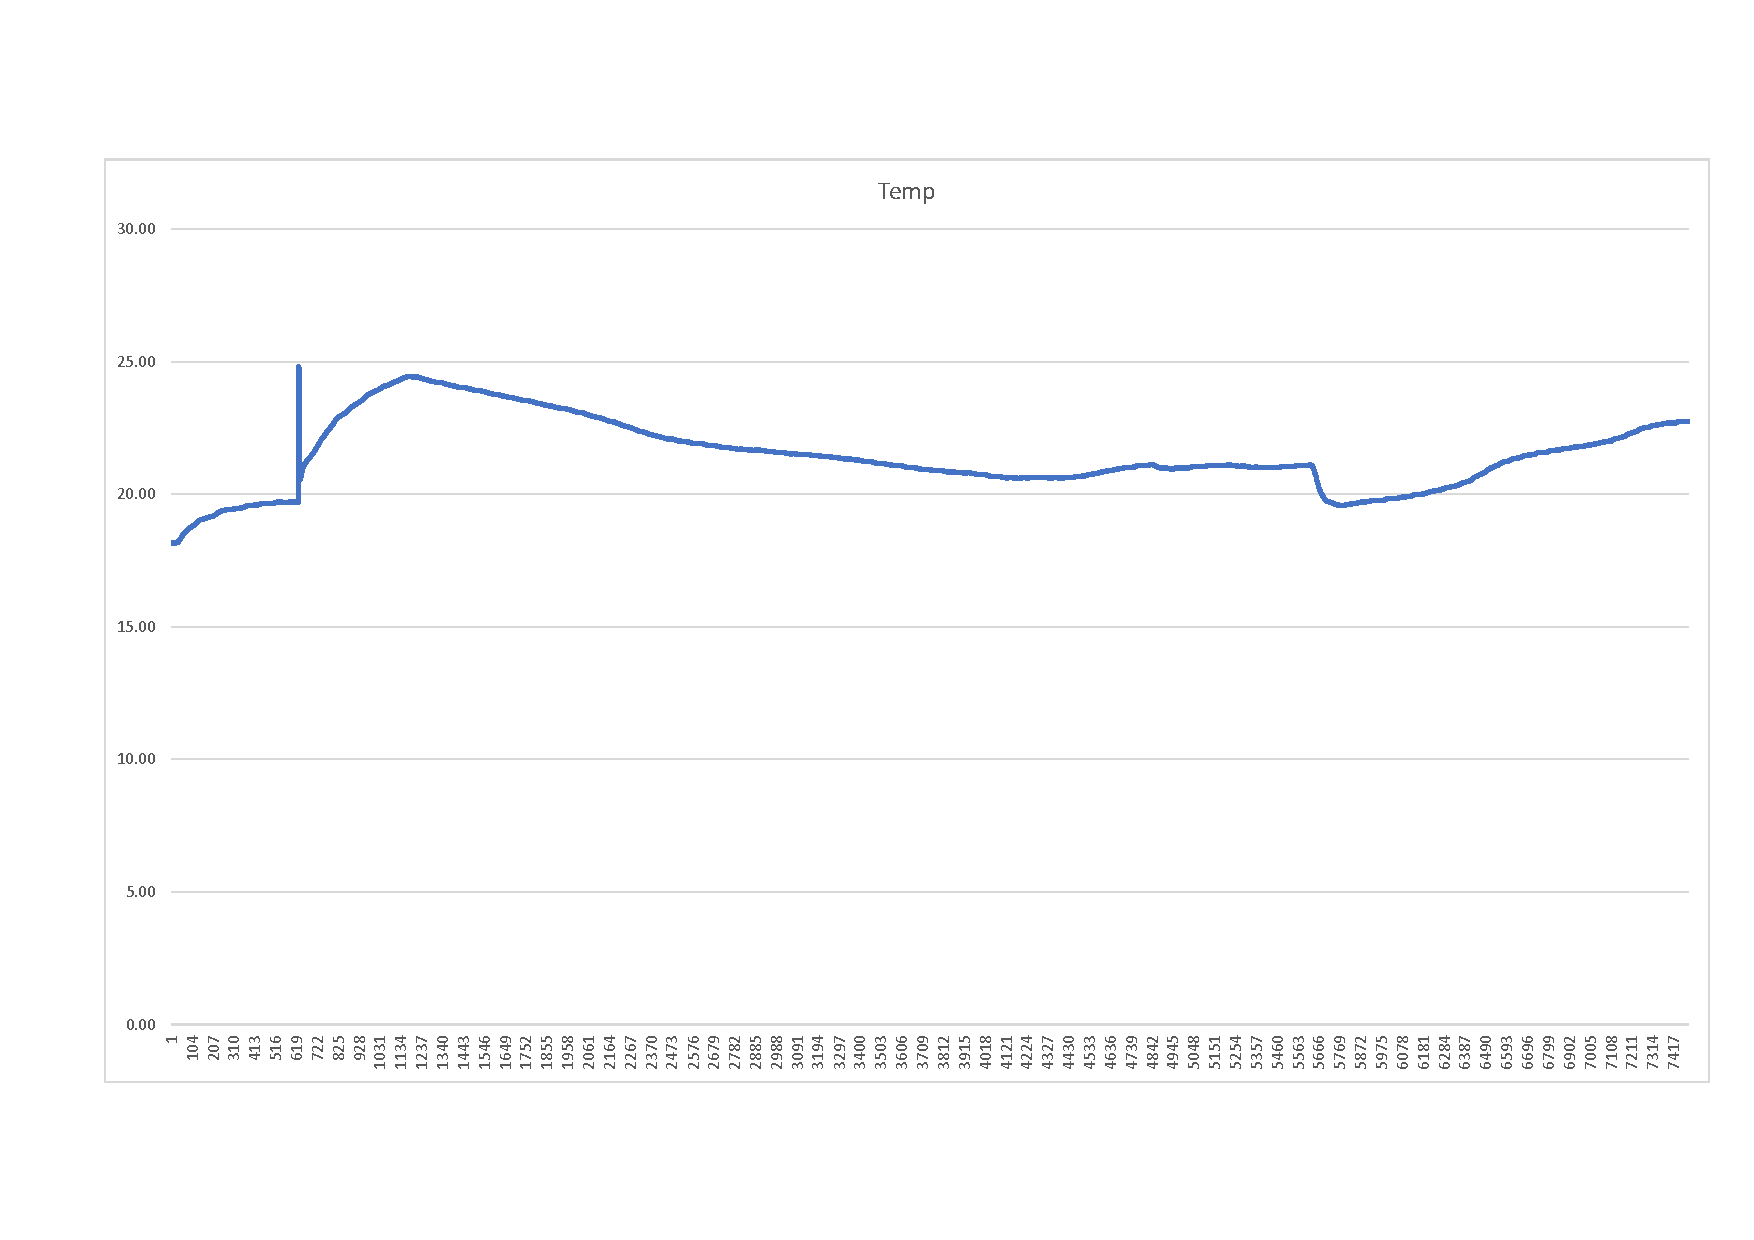
\includegraphics[width=\textwidth]{body/fig/Temp.pdf}%
%	\caption{Temperature}
%	\label{fig:temp}
%	\endminipage\hfill
%	\minipage{0.45\textwidth}%
%	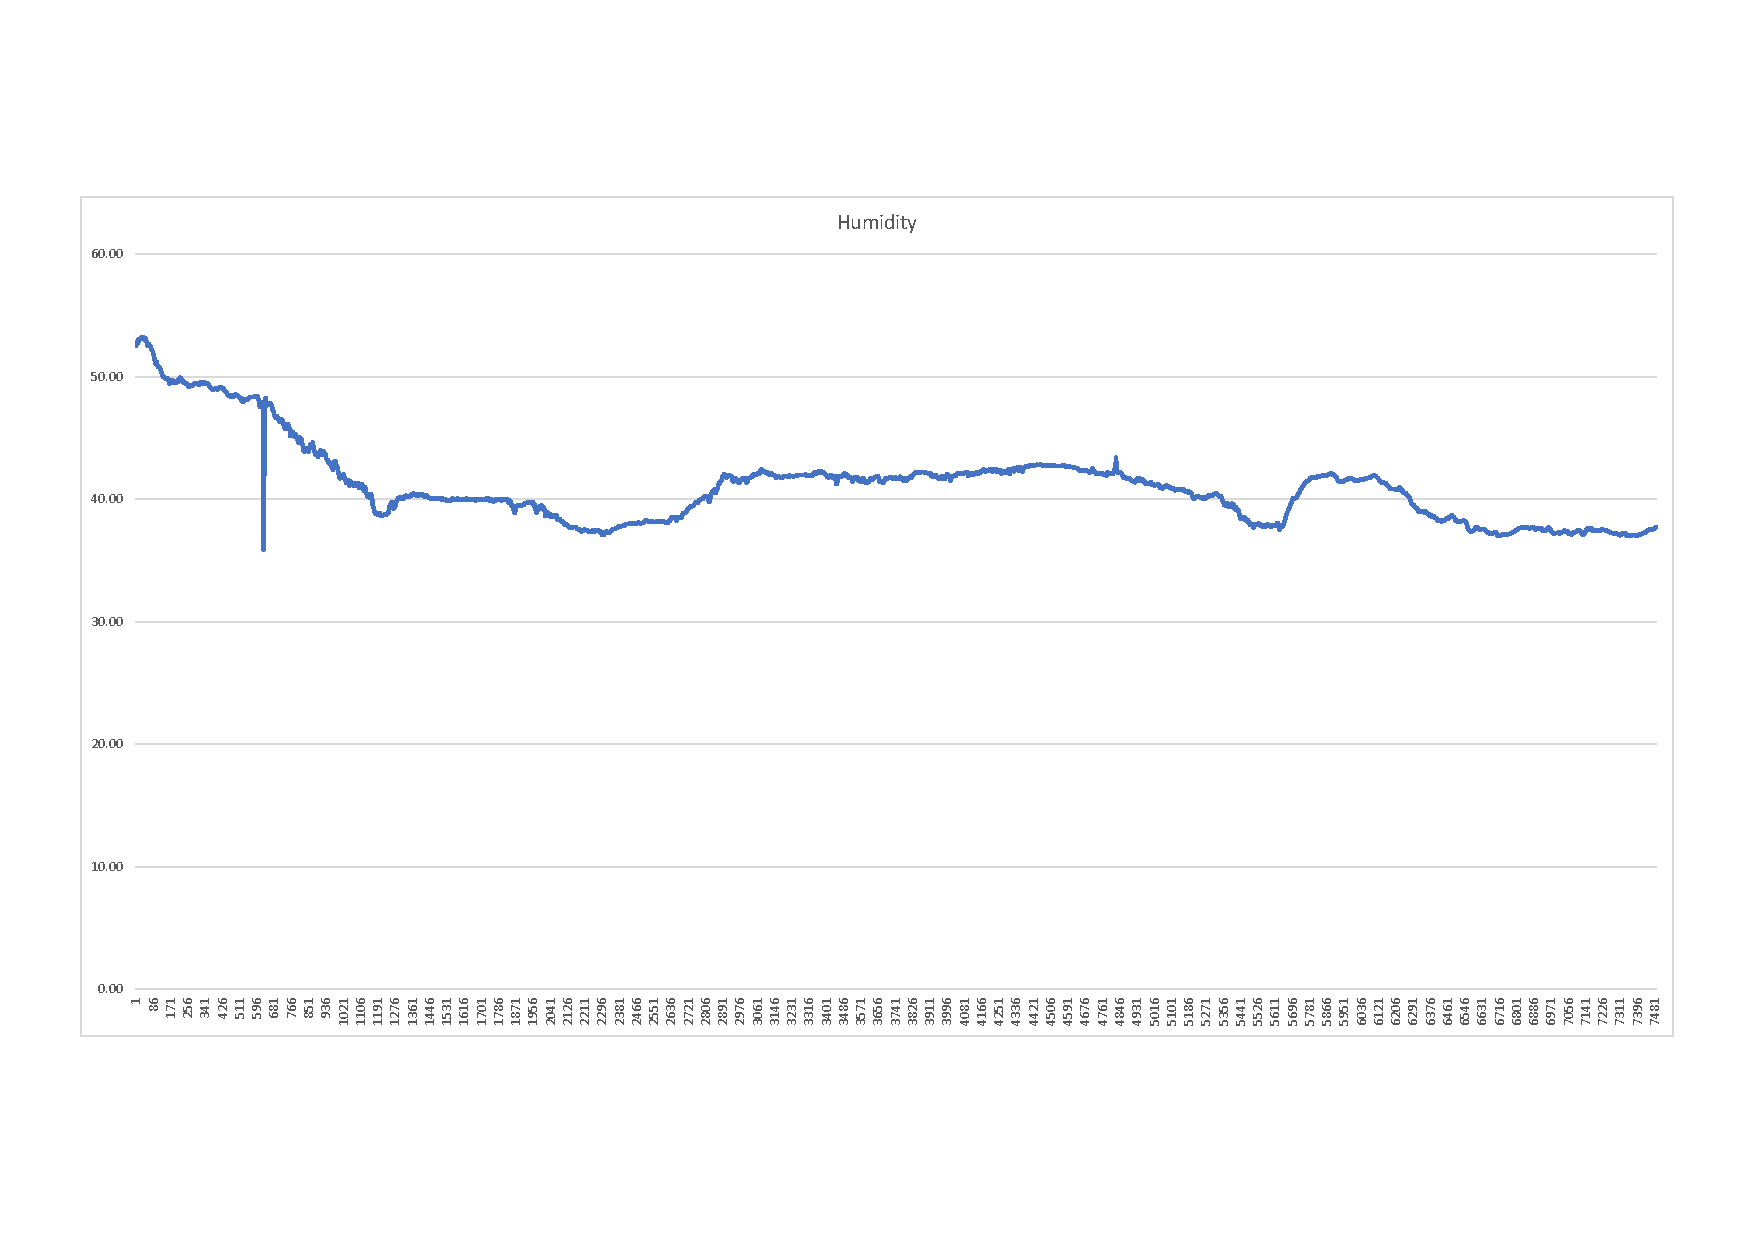
\includegraphics[width=\textwidth]{body/fig/hum.pdf}%
%	\captionof{figure}{Humidity}
%	\label{fig:hum}
%	\endminipage\hfill
%	
%	%\text{Charts provided by \cite{2007Comparison}}
%\end{figure}